\documentclass{standalone}
\usepackage{tikz}
\begin{document}
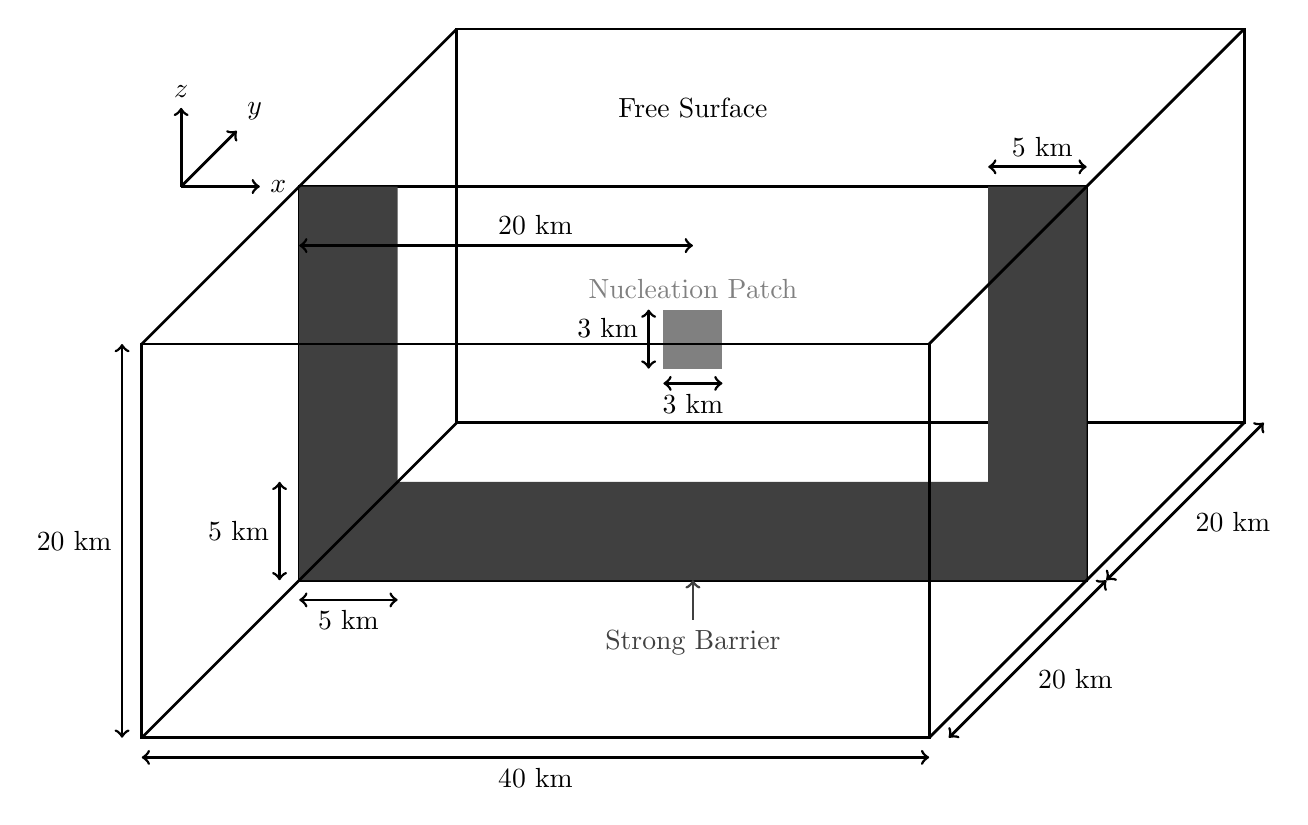
\begin{tikzpicture}[line width=1pt]
\draw (2, 2) rectangle (12, 7);
\draw (4, 4) rectangle (14, 9);
\draw[line width=1pt,<->] (0,-0.25) -- (5,-0.25) node[anchor=north]{40 km} -- (10, -0.25);
\draw[line width=1pt,<->] (-0.25,0) -- (-0.25,2.5) node[anchor=east]{20 km} -- (-0.25, 5);
\draw[line width=1pt,<->] (10.25,0) -- (11.25,1) node[anchor=north west]{20 km} -- (12.25, 2);
\draw[line width=1pt,<->] (12.25,2) -- (13.25,3) node[anchor=north west]{20 km} -- (14.25, 4);
\fill[color=darkgray] (2,2) -- (12, 2) -- (12, 7) -- (10.75, 7) -- (10.75, 3.25) -- (3.25, 3.25) -- (3.25, 7) -- (2, 7) -- (2,2);
\draw[line width=1pt,<->] (2,1.75) -- (2.625,1.75) node[anchor=north]{5 km} -- (3.25, 1.75);
\draw[line width=1pt,<->] (10.75,7.25) -- (11.4375, 7.25) node[anchor=south]{5 km} -- (12, 7.25);
\draw[line width=1pt,<->] (1.75,2) -- (1.75,2.625) node[anchor=east]{5 km} -- (1.75, 3.25);
\fill[color=gray] (6.625,4.6875) rectangle (7.375, 5.4375);
\draw[color=gray] (7,5.4375) node[anchor=south]{Nucleation Patch};
\draw[line width=1pt,<->] (6.625,4.5) -- (7,4.5) node[anchor=north]{3 km} -- (7.375, 4.5);
\draw[line width=1pt,<->] (6.4375,4.6875) -- (6.4375,5.2) node[anchor=east]{3 km} -- (6.4375, 5.4375);
\draw[line width=1pt,<->] (2,6.25) -- (5,6.25) node[anchor=south]{20 km} -- (7, 6.25);
\draw[line width=1pt,->] (0.5,7) -- (1.5,7) node[anchor=west]{$x$};
\draw[line width=1pt,->] (0.5,7) -- (1.207,7.707) node[anchor=south west]{$y$};
\draw[line width=1pt,->] (0.5,7) -- (0.5,8) node[anchor=south]{$z$};
\draw[line width=1pt, color=darkgray,->] (7,1.5) node[anchor=north]{Strong Barrier} -- (7,2);
\draw (7,8) node{Free Surface};
\draw (0,0) rectangle (10,5);
\draw (0, 0) -- (4, 4);
\draw (0, 5) -- (4, 9);
\draw (10, 0) -- (14, 4);
\draw (10, 5) -- (14, 9);
\end{tikzpicture}
\end{document}